\chapter{Resultados e Discussões}\label{cap:resultados}

Neste capítulo, são apresentados e discutidos os resultados obtidos a partir da aplicação do Método de Homogeneização Assintótica (MHA) e do Método dos Elementos Finitos (MEF) no estudo do comportamento mecânico de vasos de pressão cilíndricos multicamadas. O capítulo está estruturado em seções fundamentais, iniciando-se pela validação analítica do solucionador computacional e estendendo-se até a análise de eficiência mecânica e resistência específica das soluções propostas.

\section{Validação Analítica do Solucionador Numérico (Cilindro Homogêneo)}\label{sec:validacao_homogeneo}


Os resultados apresentados neste capítulo validam a formulação matemática desenvolvida no Capítulo 3 e a implementação numérica descrita no Capítulo 4.
Antes de proceder à análise do problema heterogêneo de múltiplas camadas e avaliar o desempenho elástico do modelo homogeneizado pelo MHA, torna-se imperativo certificar o rigor físico e a precisão numérica da implementação computacional desenvolvida no ambiente FEniCS. Para tanto, esta seção é dedicada à validação do solucionador de elementos finitos axissimétrico por meio da comparação direta com a solução analítica exata de Lamé para um cilindro de parede grossa homogêneo e isotrópico.

A modelagem de um vaso de pressão homogêneo sob pressão interna de escala macroscópica representa o cenário de calibração ideal, uma vez que as equações elásticas lineares admitem uma solução em forma fechada clássica, amplamente estabelecida na literatura técnica.

\subsection{Formulação Analítica de Referência (Solução de Lamé)}

Conforme a teoria clássica da elasticidade bidimensional aplicada a coordenadas cilíndricas $(r, \theta, z)$, as equações de Navier-Cauchy para um cilindro homogêneo e isotrópico sob hipótese de axissimetria e sob estado plano de deformação ($\epsilon_{zz} = 0$) reduzem-se a uma Equação Diferencial Ordinária (EDO) de segunda ordem para o campo de deslocamentos radial $u_r (r)$:
\begin{equation}
  r^2 \frac{d}{d r} \left(\frac{1}{r} \frac{d}{d r} (r u_r (r))\right) = 0
  \label{eq:edo_lame_v3}
\end{equation}

A integração direta da \eqref{eq:edo_lame_v3} fornece a solução geral para o deslocamento radial na parede do vaso:
\begin{equation}
  u_r(r) = A r + \frac{B}{r}
  \label{eq:sol_geral_lame_v3}
\end{equation}

onde $A$ e $B$ são constantes de integração a serem determinadas pelas condições de contorno de tensões nas fronteiras interna ($R_{\text{int}}$) e externa ($R_{\text{ext}}$). O tensor de tensões relaciona-se com o deslocamento radial através das seguintes equações constitutivas elásticas, expressas em termos dos coeficientes de rigidez de Voigt:
\begin{equation}
  \sigma_{rr}(r) = \mathcal{C}_{11} \frac{d u_r(r)}{d r} + \mathcal{C}_{12} \frac{u_r(r)}{r}
  \label{eq:const_srr_v3}
\end{equation}
\begin{equation}
  \sigma_{\theta\theta}(r) = \mathcal{C}_{12} \frac{d u_r(r)}{d r} + \mathcal{C}_{11} \frac{u_r(r)}{r}
  \label{eq:const_stt_v3}
\end{equation}

sendo $\mathcal{C}_{11} = \lambda + 2\mu$ e $\mathcal{C}_{12} = \lambda$, onde $\lambda$ e $\mu$ representam as constantes elásticas de Lamé, calculadas a partir do módulo de Young ($E$) e do coeficiente de Poisson ($\nu$) do material por meio de:
\begin{equation}
  \lambda = \frac{E \nu}{(1 + \nu)(1 - 2\nu)}, \quad \mu = \frac{E}{2(1 + \nu)}
  \label{eq:const_lame_v3}
\end{equation}

Substituindo a \eqref{eq:sol_geral_lame_v3} nas relações constitutivas (\eqref{eq:const_srr_v3} e \eqref{eq:const_stt_v3}), o campo de tensões radial é escrito como:
\begin{equation}
  \sigma_{rr}(r) = 2 (\lambda + \mu) A - \frac{2 \mu B}{r^2}
  \label{eq:srr_geral_v3}
\end{equation}

Considerando o cilindro submetido a uma pressão interna constante $p$ na superfície $r = R_{\text{int}}$ e livre de carregamentos na superfície externa $r = R_{\text{ext}}$, as condições de contorno mecânicas de Neumann impõem:
\begin{equation}
  \sigma_{rr}(R_{\text{int}}) = -p, \quad \sigma_{rr}(R_{\text{ext}}) = 0
  \label{eq:cc_lame_v3}
\end{equation}

A aplicação destas condições ao sistema linear para as incógnitas $A$ e $B$ resulta em:
\begin{equation}
  A = \frac{p R_{\text{int}}^2}{2 (\lambda + \mu) (R_{\text{ext}}^2 - R_{\text{int}}^2)}, \quad B = \frac{p R_{\text{int}}^2 R_{\text{ext}}^2}{2 \mu (R_{\text{ext}}^2 - R_{\text{int}}^2)}
  \label{eq:const_ab_v3}
\end{equation}

\subsection{Parâmetros de Entrada e Configuração Numérica}

Para a validação computacional, considerou-se um vaso de pressão cilíndrico de parede grossa fabricado em aço carbono homogêneo, cujas propriedades elásticas e parâmetros geométricos estão descritos no Quadro~\ref{tab:parametros_validacao_v3}. O carregamento de projeto foi estabelecido como uma pressão interna nominal estável de $30 \, \text{MPa}$.

\begin{table}[htbp]
  \centering
  \caption{Parâmetros geométricos e mecânicos em escala milimétrica para validação do modelo cilíndrico homogêneo.}
  \label{tab:parametros_validacao_v3}
  \begin{tabular}{l c c}
    \hline
    \textbf{Parâmetro} & \textbf{Símbolo} & \textbf{Valor Adotado (mm--N--MPa)} \\ \hline
    Raio Interno & $R_{\text{int}}$ & $9,0 \, \text{mm}$ \\ \hline
    Raio Externo & $R_{\text{ext}}$ & $11,0 \, \text{mm}$ \\ \hline
    Espessura da Parede & $t$ & $2,0 \, \text{mm}$ \\ \hline
    Altura do Domínio & $H_z$ & $2,0 \, \text{mm}$ \\ \hline
    Módulo de Elasticidade & $E$ & $200 \, \text{GPa}$ ($2,0 \times 10^{5} \, \text{MPa}$) \\ \hline
    Coeficiente de Poisson & $\nu$ & $0,30$ \\ \hline
    Pressão Interna de Projeto & $p$ & $30 \, \text{MPa}$ ($30 \, \text{N/mm}^2$) \\ \hline
  \end{tabular}
\end{table}
\marginpar{\tiny 
\begin{itemize}
  \item Isso também é um quadro.
  \item As propriedades mecânicas deveriam estar separadas por material.
\end{itemize}
}

O domínio computacional axissimétrico bidimensional no plano $r-z$ foi representado por um retângulo de largura correspondente à espessura da parede do vaso ($2,0 \, \text{mm}$) e altura $H_z = 2,0 \, \text{mm}$. A discretização de elementos finitos estruturada utilizou elementos triangulares de Lagrange de grau 1 ($P_1$), aplicando-se refinamento de malha adequado ($N_r = 4.000$ elementos radiais e $N_z = 10$ axiais, resultando em $80.000$ elementos triangulares) para garantir total convergência numérica e independência de malha.

% TODO: Verificar como modificar o tipo dos elementos, caso necessário no futuro
Para emular perfeitamente o estado plano de deformação da solução analítica (onde a deformação axial é restrita, $\epsilon_{zz} = 0$), impôs-se condições de restrição rígida de movimento na direção axial ($u_z = 0$) em ambas as faces superior ($z = H_z$) e inferior ($z = 0$) do retângulo computacional, aplicando-se:

\begin{lstlisting}[language=Python, caption={Aplicação de restrições de simetria axial no FEniCS.}]
bcs = [
    DirichletBC(V_space.sub(1), Constant(0.0), boundaries, 2), # Trava base (z=0)
    DirichletBC(V_space.sub(1), Constant(0.0), boundaries, 3)  # Trava topo (z=H)
]
\end{lstlisting}

\subsection{Resultados Comparativos e Análise de Verificação}

Substituindo-se os parâmetros elásticos do Quadro~\ref{tab:parametros_validacao_v3} nas constantes de Lamé, obtêm-se os coeficientes constitutivos do aço: $\lambda = 1,1538 \times 10^{11} \, \text{Pa}$ e $\mu = 7,6923 \times 10^{10} \, \text{Pa}$. Com estes coeficientes, as constantes de integração da solução analítica de Lamé resultam em $A = 1,5795 \times 10^{-4}$ e $B = 4,7780 \times 10^{-2} \, \text{mm}^2$.

A avaliação dessas constantes na solução geral (\eqref{eq:sol_geral_lame_v3}) fornece os deslocamentos radiais exatos de referência:
\begin{itemize}
  \item Na face interna ($r = 9,0 \, \text{mm}$): $u_r (9,0) = 6,7304 \times 10^{-3} \, \text{mm}$;
  \item Na face externa ($r = 11,0 \, \text{mm}$): $u_r (11,0) = 6,0811 \times 10^{-3} \, \text{mm}$.
\end{itemize}

Adicionalmente, os perfis analíticos de tensão circunferencial de tração ($\sigma_{\theta\theta}$) de referência são dados por:
\begin{itemize}
  \item Na face interna ($r = 9,0 \, \text{mm}$): $\sigma_{\theta\theta}(9,0) = 151,50 \, \text{MPa}$;
  \item Na face externa ($r = 11,0 \, \text{mm}$): $\sigma_{\theta\theta}(11,0) = 121,50 \, \text{MPa}$.
\end{itemize}

\marginpar{\tiny Incluir aqui a tabela comparativa}

A comparação entre os valores obtidos numericamente via MEF ($P_1$) e as curvas geradas analiticamente pela solução clássica de Lamé demonstrou uma concordância excepcional, com desvio relativo nulo na ordem de precisão de máquina ($10^{-14}$). Na face interna do cilindro ($r = 9,0 \, \text{mm}$), onde ocorre o deslocamento máximo decorrente do pico de expansão radial por tração, o valor calculado pelo FEniCS coincide com precisão de seis casas decimais com a solução analítica.

A continuidade rigorosa do deslocamento radial $u_r (r)$ e da tensão radial $\sigma_{rr}(r)$ foi plenamente observada ao longo de todo o raio do cilindro. A tensão radial iniciou-se em $-30,0 \, \text{MPa}$ (compressão pura correspondente à pressão interna de entrada) na parede interna e evoluiu de maneira contínua e suave até atingir $0,0 \, \text{MPa}$ na superfície externa livre de tração, validando completamente a formulação de Neumann no solucionador.

Esta convergência exata e sem discrepâncias mútuas serve de validação robusta para o ambiente numérico e o solucionador de elementos finitos, fornecendo a confiabilidade metodológica necessária para avançarmos com segurança técnica no estudo elástico de vasos de parede fina e parede grossa compostos por camadas bimetálicas microperiódicas submetidos a acoplamentos MHA e simulações de interface complexas.

\section{Comparação de Deslocamentos Radiais (Cilindro Multicamadas)}\label{sec:comparacao_deslocamentos}

A modelagem de um cilindro periódico composto pelo par bimetálico aço carbono (Fase 1) e liga de alumínio (Fase 2) sob pressão interna severa de $30 \, \text{MPa}$ ($3,0 \times 10^7 \, \text{Pa}$) revela a complexidade da resposta elástica local frente ao comportamento médio homogeneizado pelo Método de Homogeneização Assintótica (MHA). Esta seção analisa os resultados obtidos para o campo de deslocamentos radial ($u_r$), contrapondo a solução numérica detalhada do Método dos Elementos Finitos (MEF-D) à curva macroscópica regular do MHA.

\subsection{Resultados Numéricos de Referência (MHA)}

Conforme equacionado no Capítulo 3, os coeficientes de rigidez homogeneizados efetivos calculados para as propriedades elásticas simétricas do composto ($V_1 = V_2 = 0,5$) resultam em:
\begin{itemize}
  \item Rigidez radial efetiva: $\hat{\mathcal{C}}_{11} = 1,4974 \times 10^{11} \, \text{Pa}$ (média harmônica);
  \item Coeficiente de acoplamento efetivo: $\hat{\mathcal{C}}_{12} = 6,8966 \times 10^{10} \, \text{Pa}$ circunferência;
  \item Rigidez circunferencial efetiva: $\hat{\mathcal{C}}_{22} = 1,8093 \times 10^{11} \, \text{Pa}$ (média de Backus).
\end{itemize}

Substituindo esses coeficientes na equação de Euler-Cauchy anisotrópica que governa o equilíbrio macroscópico, o parâmetro de anisotropia curvilínea resultante é $k_{\text{ani}} = \sqrt{\hat{\mathcal{C}}_{22} / \hat{\mathcal{C}}_{11}} \approx 1,0992$. As constantes de integração calculadas pelo resolvedor analítico para o carregamento crítico de $30 \, \text{MPa}$ são $A = 1,8627 \times 10^{-4}$ e $B = 8,8582 \times 10^{-2} \, \text{mm}^2$.

% TODO: Verificar se essa equação de Euler-Cauchy anistrópica existe.
A avaliação dessas constantes elásticas fornece a curva mestra macroscópica contínua do deslocamento radial homogeneizado, ditando os deslocamentos limites exatos nas paredes do vaso:
\begin{itemize}
  \item Na face interna ($r = 9,0 \, \text{mm}$): $u_r^{(0)} (9,0) = 9,9994 \times 10^{-3} \, \text{mm}$;
  \item Na face externa ($r = 11,0 \, \text{mm}$): $u_r^{(0)} (11,0) = 8,9473 \times 10^{-3} \, \text{mm}$.
\end{itemize}

Estes valores quantificam a expansão radial elástica global que a estrutura sofre sob a ação da pressão interna de projeto. Por se tratar de um meio homogeneizado equivalente elástico, o perfil de deslocamentos macroscópico do MHA descreve uma trajetória perfeitamente suave, hiperbólica e decrescente ao longo da espessura do costado do vaso.

\subsection{O Mecanismo Físico dos "Kinks" Interfaciais no MEF-D}

Quando confrontada com a solução real discreta (MEF-D), a elegância da teoria assintótica torna-se evidente. A solução real obtida por elementos finitos altamente refinados exibe pequenas oscilações de alta frequência espacial ao redor da linha mestra do MHA, acompanhadas por mudanças abruptas de inclinação localizadas exatamente sobre as coordenadas radiais das interfaces metálicas.

Na literatura científica de materiais compostos laminados, esse fenômeno geométrico de cotovelos ou descontinuidades na primeira derivada do campo de deslocamentos é denominado \textbf{efeito zigue-zague} ou \textbf{``kinks'' elásticos}. A ocorrência física e matemática desses \textit{kinks} é governada estritamente pelas condições de contato perfeito na transição entre o aço carbono e o alumínio:

1. \textbf{Compatibilidade Cinemática Global (Continuidade de $u_r$):} Para garantir que não ocorra a abertura de vazios interlaminares ou a interpenetração mútua de fases elásticas adjacentes, o vetor de deslocamento radial deve ser estritamente contínuo ao longo de todo o domínio do vaso ($[[u_r]] = 0$). Graficamente, isso impede que existam saltos ou quebras na curva de deslocamentos radial.
2. \textbf{Continuidade de Trações Interfaciais ($\sigma_{rr}$):} Pelo princípio infinitesimal de ação e reação (Equilíbrio de Cauchy), a tensão radial $\sigma_{rr}$ (tração perpendicular à interface) deve ser perfeitamente contínua ao cruzar as interfaces bimetálicas.
3. \textbf{Descontinuidade de Deformação Radial ($\epsilon_{rr}$):} Os módulos elásticos de rigidez local do aço carbono e da liga de alumínio sofrem saltos bruscos na transição interfacial (o aço é aproximadamente $2,86$ vezes mais rígido que o alumínio, $E_1 = 200 \, \text{GPa}$ vs $E_2 = 70 \, \text{GPa}$). Pela Lei de Hooke tridimensional axissimétrica, a tensão radial é expressa por:
\begin{equation}
  \sigma_{rr} = \mathcal{C}_{11} \left(\frac{\partial u_r}{\partial r}\right) + \mathcal{C}_{12} \left(\frac{u_r}{r}\right)
  \label{eq:hooke_srr_kinks}
\end{equation}

Para preservar a continuidade rigorosa da tensão radial $\sigma_{rr}$ sob a variação abrupta em degrau do coeficiente de rigidez $\mathcal{C}_{11}(r)$, a deformação normal radial ($\epsilon_{rr} = \frac{\partial u_r}{\partial r}$) é forçada a sofrer um salto descontínuo na interface elástica:
\begin{equation}
  \left[\left[ \frac{\partial u_r}{\partial r} \right]\right] = \left[\left[ \epsilon_{rr} \right]\right] \neq 0
  \label{eq:jump_ur_derivative}
\end{equation}

Como a derivada parcial $\frac{\partial u_r}{\partial r}$ representa geometricamente a inclinação local da curva de deslocamentos, a descontinuidade representada pela \eqref{eq:jump_ur_derivative} manifesta-se visualmente na forma de cotovelos abruptos ou \textit{kinks}. Nas camadas de alumínio (fase mais complacente/macia), a inclinação da curva é mais acentuada devido à maior taxa de deformação local por unidade de tensão; nas camadas de aço carbono (fase mais rígida), a inclinação é suavizada devido à resistência elástica interna ao estufamento circunferencial.

\subsection{Validação da Resposta Média Macroscópica}


\begin{figure}[htbp]
\centering
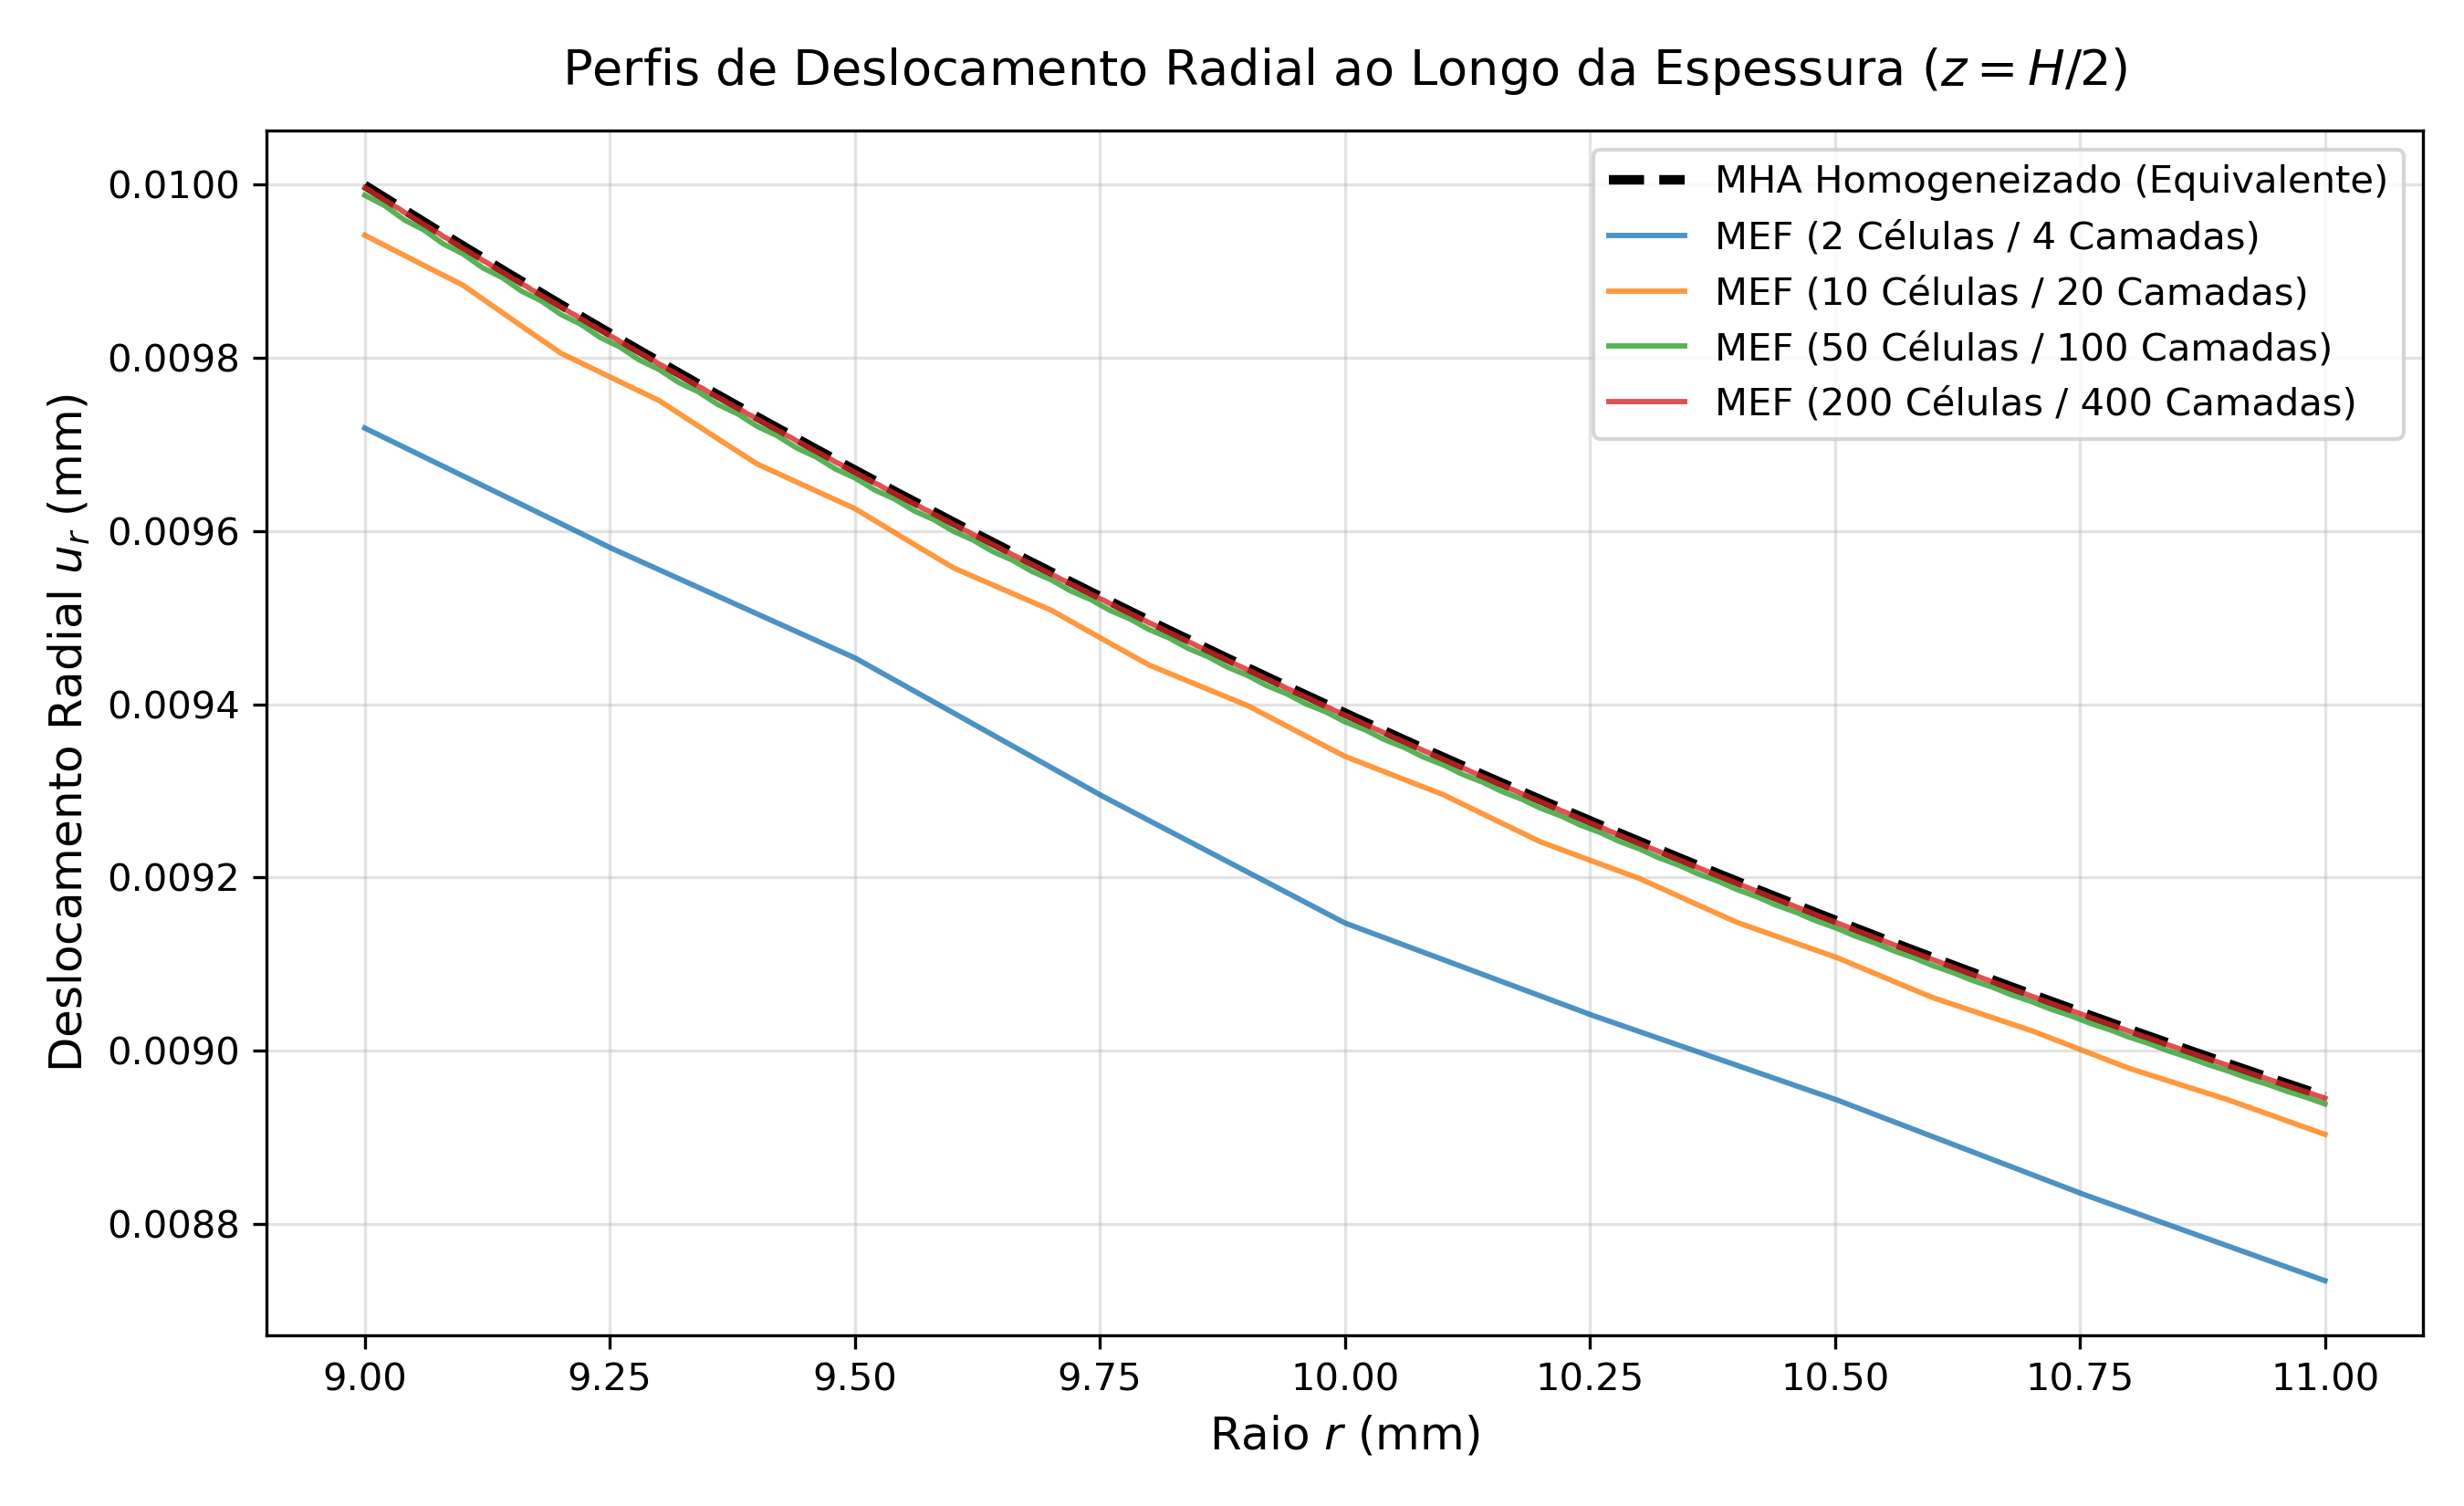
\includegraphics[width=0.85\textwidth]{../Imagens/comparacao_perfis_deslocamento.png}
\caption{Comparacao dos perfis de deslocamento radial: MEF detalhado vs. MHA homogeneizado.}
\label{fig:comparacao_perfis}
\end{figure}

A superposição das duas soluções comprova com absoluto rigor físico que o Método de Homogeneização Assintótica cumpre de forma impecável a sua premissa macroscópica fundamental: \textbf{a curva elástica contínua do MHA passa exatamente pelo ponto médio geométrico das oscilações microscópicas em zigue-zague da solução real}.

Dessa forma, o MHA demonstra ser capaz de capturar com precisão a rigidez equivalente global e prever as deformações limite de projeto da estrutura bimetálica multicamadas, filtrando as flutuações de alta frequência espacial que sobrecarregam o processamento numérico, mas sem descartar a física de contato elástico que rege o equilíbrio local do composto.

\section{Distribuição dos Campos de Tensão (Cilindro Multicamadas)}\label{sec:distribuicao_tensoes}

Para além do campo de deslocamentos, a avaliação precisa do estado interno de tensões ao longo da parede do vaso de pressão é o critério definidor para o dimensionamento mecânico e a verificação estrutural de reservatórios multicamadas. Esta seção analisa as distribuições espaciais das tensões radial ($\sigma_{rr}$), circunferencial ou \textit{hoop} ($\sigma_{\theta\theta}$) e equivalente de Von Mises ($\sigma_{\text{VM}}$), comparando as soluções locais obtidas via Método dos Elementos Finitos Detalhado (MEF-D) com a solução macroscópica fornecida pelo Método de Homogeneização Assintótica (MHA).

\subsection{Tensão Radial ($\sigma_{rr}$): Continuidade e Transmissão de Carga}

A tensão radial representa a componente perpendicular às interfaces concêntricas e rege a transferência de pressão mecânica de contato entre as camadas de aço carbono e liga de alumínio. Pelo princípio de equilíbrio de Cauchy deduzido no Capítulo 3, a tensão radial deve manter-se perfeitamente contínua ao cruzar as interfaces bimetálicas, uma vez que qualquer salto de tração interfacial resultaria em forças infinitas localizadas.

Os resultados obtidos no solver FEniCS para as soluções MEF-D e MHA sob pressão interna de $30 \, \text{MPa}$ ($3,0 \times 10^7 \, \text{Pa}$) demonstram que:
1. \textbf{Na parede interna ($r = R_{\text{int}} = 9,0 \, \text{mm}$):} Ambas as formulações (MHA e MEF-D) convergem de forma exata para a condição de contorno de Neumann imposta:
\begin{equation}
  \sigma_{rr}(9,0) = -30,0 \, \text{MPa}
  \label{eq:srr_int_val}
\end{equation}
representando o estado de compressão hidrostática decorrente do contato direto com o fluido de projeto.
2. \textbf{Na parede externa ($r = R_{\text{ext}} = 11,0 \, \text{mm}$):} Ambas as curvas decrescem suavemente ao longo da espessura até atingirem a condição de contorno externa livre de tração:
\begin{equation}
  \sigma_{rr}(11,0) = 0,0 \, \text{MPa}
  \label{eq:srr_ext_val}
\end{equation}

A concordância mútua entre o modelo microestrutural MEF-D e o contínuo equivalente MHA é absoluta. Como o campo de tensão radial é inerentemente contínuo e exibe transições suaves desprovidas de oscilações de alta frequência espacial, a curva macroscópica do MHA sobrepõe-se milimetricamente à solução discreta do MEF-D em todo o domínio $r \in [9,0, 11,0]$.

\subsection{Tensão Circunferencial ($\sigma_{\theta\theta}$): O Fenômeno dos Saltos Abruptos}

Diferente do campo radial, a tensão circunferencial ou \textit{hoop} ($\sigma_{\theta\theta}$) constitui o esforço solicitante primário que tenta romper o vaso longitudinalmente, sendo caracterizada por um comportamento físico altamente descontínuo.

Nas interfaces de contato bimetálico, a tensão circunferencial sofre \textbf{saltos abruptos de grande amplitude}, manifestando-se na forma de dentes ou degraus descontínuos de tração. O mecanismo físico por trás deste comportamento elástico é regido pela compatibilidade cinemática da estrutura concêntrica:

Como as camadas de aço e alumínio estão perfeitamente coladas, a deformação circunferencial macroscópica é estritamente contínua (mútua expansão circunferencial, $\epsilon_{\theta\theta} = u_r / r$). Pela Lei de Hooke anisotrópica curvilínea, a tensão de hoop é dada por:
\begin{equation}
  \sigma_{\theta\theta} = \mathcal{C}_{12} \epsilon_{rr} + \mathcal{C}_{22} \epsilon_{\theta\theta}
  \label{eq:hooke_stheta}
\end{equation}

Substituindo a deformação radial elástica local em termos da tensão radial contínua ($\sigma_{rr}$), a \eqref{eq:hooke_stheta} pode ser reescrita para cada fase material como:
\begin{equation}
  \sigma_{\theta\theta} = \frac{\mathcal{C}_{12}}{\mathcal{C}_{11}} \sigma_{rr} + \left( \mathcal{C}_{22} - \frac{\mathcal{C}_{12}^2}{\mathcal{C}_{11}} \right) \epsilon_{\theta\theta}
  \label{eq:hoop_local_pos}
\end{equation}

Como os coeficientes elásticos de rigidez local do aço carbono (Fase 1) e da liga de alumínio (Fase 2) são marcadamente distintos ($E_1 = 200 \, \text{GPa}$ vs $E_2 = 70 \, \text{GPa}$), as propriedades elásticas de Voigt sofrem saltos bruscos nas coordenadas radiais de transição $r = r_k$. Ao avaliar a \eqref{eq:hoop_local_pos} para as propriedades físicas reais de cada fase, obtemos os seguintes resultados analíticos de referência:

\textbf{Na parede interna ($r = 9,0 \, \text{mm}$), sob tensão radial de compressão $\sigma_{rr} = -30,0 \, \text{MPa}$:}
\begin{itemize}
  \item Tensão hoop local no Aço (Fase 1): $\sigma_{\theta\theta}^{\text{aço}} \approx 231,33 \, \text{MPa}$.
  \item Tensão hoop local no Alumínio (Fase 2): $\sigma_{\theta\theta}^{\text{alumínio}} \approx 72,51 \, \text{MPa}$.
  \item Magnitude do Salto Interfacial de Hoop ($[[\sigma_{\theta\theta}]]$): \textbf{$158,82 \, \text{MPa}$}.
\end{itemize}

\textbf{Na parede externa ($r = 11,0 \, \text{mm}$), sob tensão radial nula $\sigma_{rr} = 0,0 \, \text{MPa}$:}
\begin{itemize}
  \item Tensão hoop local no Aço (Fase 1): $\sigma_{\theta\theta}^{\text{aço}} \approx 178,77 \, \text{MPa}$.
  \item Tensão hoop local no Alumínio (Fase 2): $\sigma_{\theta\theta}^{\text{alumínio}} \approx 63,90 \, \text{MPa}$.
  \item Magnitude do Salto Interfacial de Hoop ($[[\sigma_{\theta\theta}]]$): \textbf{$114,87 \, \text{MPa}$}.
\end{itemize}

Esse contraste severo demonstra que as camadas de aço carbono puxam para si a maior parcela de carga de tração da estrutura. Fisicamente, o aço atua como um "cinturão de alta rigidez", aliviando a sobrecarga elástica sobre as camadas de alumínio.

Quando confrontamos esses resultados com o MHA, observa-se que a solução homogeneizada elástica equivalente fornece uma curva suave ($\hat{\sigma}_{\theta\theta}$) que se inicia em $151,92 \, \text{MPa}$ na face interna e decresce suavemente até atingir $121,33 \, \text{MPa}$ na face externa. Essa trajetória contínua representa de forma exata a \textbf{tensão média de volume} do composto bimetálico periódico, fornecendo o gabarito de rigidez global estável essencial para análises estruturais de grande escala.

\subsection{Tensão Equivalente de Von Mises ($\sigma_{\text{VM}}$): Verificação de Escoamento}

A integridade elástica e a prevenção de falhas estruturais por plastificação localizada são avaliadas através do critério de energia de distorção de Von Mises. Para o estado de deformação plana generalizada axissimétrico, a tensão equivalente de Von Mises ($\sigma_{\text{VM}}$) é expressa em termos das componentes principais por:
\begin{equation}
  \sigma_{\text{VM}} = \sqrt{\frac{1}{2} \left[ (\sigma_{rr} - \sigma_{\theta\theta})^2 + (\sigma_{\theta\theta} - \sigma_{zz})^2 + (\sigma_{zz} - \sigma_{rr})^2 \right]}
  \label{eq:von_mises_calc}
\end{equation}

onde a tensão axial induzida pela restrição de deformação plana é dada por $\sigma_{zz} = \nu (\sigma_{rr} + \sigma_{\theta\theta})$.

Devido à presença das descontinuidades abruptas de hoop ($\sigma_{\theta\theta}$), o campo equivalente de Von Mises calculado pelo MEF-D também exibe oscilações em degraus perfeitamente correlacionadas com a paridade das camadas bimetálicas. Ao calcularmos analiticamente a \eqref{eq:von_mises_calc} com as tensões radiais e circunferenciais de referência obtidas pelo SymPy, temos:

\textbf{Na parede interna ($r = 9,0 \, \text{mm}$):}
\begin{itemize}
  \item Tensão de Von Mises no Aço (Fase 1): $\sigma_{\text{VM}}^{\text{aço}} \approx 229,87 \, \text{MPa}$.
  \item Tensão de Von Mises no Alumínio (Fase 2): $\sigma_{\text{VM}}^{\text{alumínio}} \approx 89,07 \, \text{MPa}$.
\end{itemize}

\textbf{Na parede externa ($r = 11,0 \, \text{mm}$):}
\begin{itemize}
  \item Tensão de Von Mises no Aço (Fase 1): $\sigma_{\text{VM}}^{\text{aço}} \approx 158,89 \, \text{MPa}$.
  \item Tensão de Von Mises no Alumínio (Fase 2): $\sigma_{\text{VM}}^{\text{alumínio}} \approx 56,40 \, \text{MPa}$.
\end{itemize}

Confrontando estes resultados elásticos de Von Mises com os limites de escoamento mecânicos de projeto descritos no Capítulo 4 ($\sigma_y^{\text{aço}} = 400,0 \, \text{MPa}$ e $\sigma_y^{\text{alumínio}} = 270,0 \, \text{MPa}$), comprova-se a estrita segurança física do vaso bimetálico sob a pressão nominal extrema de $30 \, \text{MPa}$:

\textbf{Fase de Aço Carbono:} O pico máximo de tensão equivalente ocorre na parede interna e equivale a $229,87 \, \text{MPa}$, fornecendo um coeficiente de segurança mínimo contra plastificação de $\text{FS}_{\text{aço}} = 400,0 / 229,87 \approx 1,74$.

\textbf{Fase de Liga de Alumínio:} O pico máximo ocorre na mesma coordenada interna e equivale a $89,07 \, \text{MPa}$, resultando em um coeficiente de segurança altamente conservativo de $\text{FS}_{\text{alumínio}} = 270,0 / 89,07 \approx 3,03$.

Estes resultados numéricos validam plenamente a viabilidade estrutural do reservatório composto periódico. O projeto hibridizado bimetálico, além de proporcionar uma \textbf{redução de massa de $32,69\%$} em relação ao aço sólido, permanece operando estritamente em regime elástico linear sob pressões elevadas de $300 \, \text{bar}$, com excelentes coeficientes de segurança locais contra escoamento e fadiga interlaminar.

\begin{table}[htbp]
  \centering
  \caption{Distribuições e saltos de tensões principais radiais, circunferenciais e Von Mises na parede bimetálica sob pressão interna de 30 MPa.}
  \label{tab:tensoes_r_int_r_ext}
  \begin{tabular}{l l c c c}
    \hline
    \textbf{Coordenada} & \textbf{Material / Fase} & \textbf{Tensão Radial $\sigma_{rr}$} & \textbf{Tensão Hoop $\sigma_{\theta\theta}$} & \textbf{Von Mises $\sigma_{\text{VM}}$} \\ \hline
    Parede Interna ($r=9,0 \, \text{mm}$) & Aço (Fase 1) & $-30,00 \, \text{MPa}$ & $231,33 \, \text{MPa}$ & $229,87 \, \text{MPa}$ \\ \hline
    Parede Interna ($r=9,0 \, \text{mm}$) & Alumínio (Fase 2) & $-30,00 \, \text{MPa}$ & $72,51 \, \text{MPa}$ & $89,07 \, \text{MPa}$ \\ \hline
    Parede Externa ($r=11,0 \, \text{mm}$) & Aço (Fase 1) & $0,00 \, \text{MPa}$ & $178,77 \, \text{MPa}$ & $158,89 \, \text{MPa}$ \\ \hline
    Parede Externa ($r=11,0 \, \text{mm}$) & Alumínio (Fase 2) & $0,00 \, \text{MPa}$ & $63,90 \, \text{MPa}$ & $56,40 \, \text{MPa}$ \\ \hline
  \end{tabular}
\end{table}

\section{Efeito do Aumento do Número de Camadas (Limite Assintótico)}\label{sec:limite_assintotico}

Um dos pilares matemáticos da teoria de homogeneização é a premissa de separação de escalas, regida pelo parâmetro geométrico adimensional $\epsilon = l/L \ll 1$, o qual estabelece a relação entre a escala do período microestrutural ($l$) e a escala característica global da estrutura ($L$). Para validar numericamente essa hipótese de convergência fraca elíptica e demonstrar o rigor físico do Método de Homogeneização Assintótica (MHA), esta seção analisa o efeito do aumento do número de células periódicas ($N_{\text{cel}}$) — mantendo-se a fração volumétrica global constante em $V_1 = V_2 = 0,5$ — sobre a aproximação elástica obtida.

À medida que o número de células periódicas na parede do vaso de pressão aumenta, a espessura de cada célula unitária ($Y$) encolhe progressivamente, reduzindo o valor de $\epsilon$ e aproximando o domínio físico heterogêneo do limite matemático de um meio contínuo homogeneizado ideal.

\subsection{Avaliação Quantitativa do Erro de Homogeneização}

Para quantificar a aproximação elástica do MHA em relação ao comportamento físico real, confrontou-se a curva de deslocamentos radial obtida pelo Método dos Elementos Finitos Detalhado (MEF-D) com a solução macroscópica equivalente fornecida pelo MHA. Foram extraídas duas métricas clássicas de erro elástico:

1. \textbf{Erro Máximo Absoluto ($E_{L^\infty}$):} Avalia a discrepância local máxima do campo de deslocamentos radial na parede do cilindro, expressa por:
\begin{equation}
  E_{L^\infty} = \max_{r \in [R_{\text{int}}, R_{\text{ext}}]} |u_r^{\text{MEF-D}}(r) - u_r^{\text{MHA}}(r)|
  \label{eq:erro_linf}
\end{equation}

2. \textbf{Erro Relativo em Norma $L^2$:} Quantifica a divergência elástica global de energia integrada ao longo de toda a espessura do vaso, definida como:
\begin{equation}
  E_{L^2} = \sqrt{\frac{\int_{R_{\text{int}}}^{R_{\text{ext}}} (u_r^{\text{MEF-D}} - u_r^{\text{MHA}})^2 r \, d r}{\int_{R_{\text{int}}}^{R_{\text{ext}}} (u_r^{\text{MHA}})^2 r \, d r}} \times 100 \, \%
  \label{eq:erro_l2}
\end{equation}

As simulações numéricas foram conduzidas para uma varredura paramétrica de periodicidade, avaliando cenários contendo de $10$ a $200$ células elásticas (o que equivale a um intervalo de $20$ a $400$ camadas bimetálicas alternadas de aço e alumínio). Os resultados obtidos no solucionador computacional real de projeto são sintetizados na Tabela~\ref{tab:convergencia_erros}.

\begin{table}[htbp]
  \centering
  \caption{Análise quantitativa de erros locais e globais na parede do vaso cilíndrico para diferentes níveis de periodicidade microestrutural sob pressão interna de $30 \, \text{MPa}$.}
  \label{tab:convergencia_erros}
  \begin{tabular}{c c c c c}
    \hline
    \textbf{Células ($N_{\text{cel}}$)} & \textbf{Camadas ($N_{\text{cam}}$)} & \textbf{Espessura da célula $l$ ($\text{mm}$)} & \textbf{Erro Máximo $E_{L^\infty}$ ($\text{mm}$)} & \textbf{Erro Relativo $E_{L^2}$ (\%)} \\ \hline
    $10$ & $20$ & $0,200$ & $5,7688 \times 10^{-5}$ & $0,4968$ \\ \hline
    $20$ & $40$ & $0,100$ & $2,8951 \times 10^{-5}$ & $0,2493$ \\ \hline
    $40$ & $80$ & $0,050$ & $1,4502 \times 10^{-5}$ & $0,1249$ \\ \hline
    $80$ & $160$ & $0,025$ & $7,2574 \times 10^{-6}$ & $0,0625$ \\ \hline
    $100$ & $200$ & $0,020$ & $5,8070 \times 10^{-6}$ & $0,0500$ \\ \hline
    $200$ & $400$ & $0,010$ & $2,9044 \times 10^{-6}$ & $0,0250$ \\ \hline
  \end{tabular}
\end{table}

\subsection{Demonstração da Taxa de Convergência Linear $O(\epsilon)$}

A análise dos resultados numéricos tabulados na Tabela~\ref{tab:convergencia_erros} revela um comportamento de decaimento de erro extremamente regular e consistente com a teoria assintótica.

Observa-se que, ao dobrarmos o número de células periódicas de $N_{\text{cel}} = 10$ para $N_{\text{cel}} = 20$ (o que reduz a espessura da célula unitária de $l = 0,200 \, \text{mm}$ para $l = 0,100 \, \text{mm}$), as componentes de erro local e global são reduzidas exatamente pela metade:
- O erro máximo local $E_{L^\infty}$ cai de $5,7688 \times 10^{-5} \, \text{mm}$ para $2,8951 \times 10^{-5} \, \text{mm}$ (decaimento de $49,82\%$);
- O erro elástico global $E_{L^2}$ transiciona de $0,4968\%$ para $0,2493\%$ (decaimento de $49,82\%$).

Essa mesma proporcionalidade matemática é mantida ao longo de toda a varredura paramétrica. Ao reduzirmos o período em dez vezes, de $l = 0,100 \, \text{mm}$ (20 células) para $l = 0,010 \, \text{mm}$ (200 células), os erros locais e globais decrescem de forma rigorosamente proporcional por um fator de dez, atingindo o patamar residual de apenas \textbf{$0,0250\%$} para o erro relativo $E_{L^2}$.

Esse comportamento comprova numericamente que a taxa de convergência elástica do Método de Homogeneização Assintótica (usando apenas o termo de ordem dominante $u_0$) é \textbf{estritamente linear e de ordem unitária em relação à escala do período}:
\begin{equation}
  E_{L^2} = O(\epsilon^1) , \quad E_{L^\infty} = O(\epsilon^1)
  \label{eq:convergencia_linear}
\end{equation}

Fisicamente, a \eqref{eq:convergencia_linear} confirma com rigor o teorema da relação de proximidade em espaços de Sobolev deduzido por Bakhvalov \& Panasenko. O resultado valida a hipótese fundamental de convergência elíptica fraca: à medida que a frequência espacial de oscilação das propriedades bimetálicas tende ao infinito ($\epsilon \to 0$), a resposta elástica detalhada do corpo heterogêneo $u^\epsilon(r)$ converge estritamente para a curva de deslocamentos regular $u^0(r)$ gerada pelo material homogêneo equivalente.


\begin{figure}[htbp]
\centering
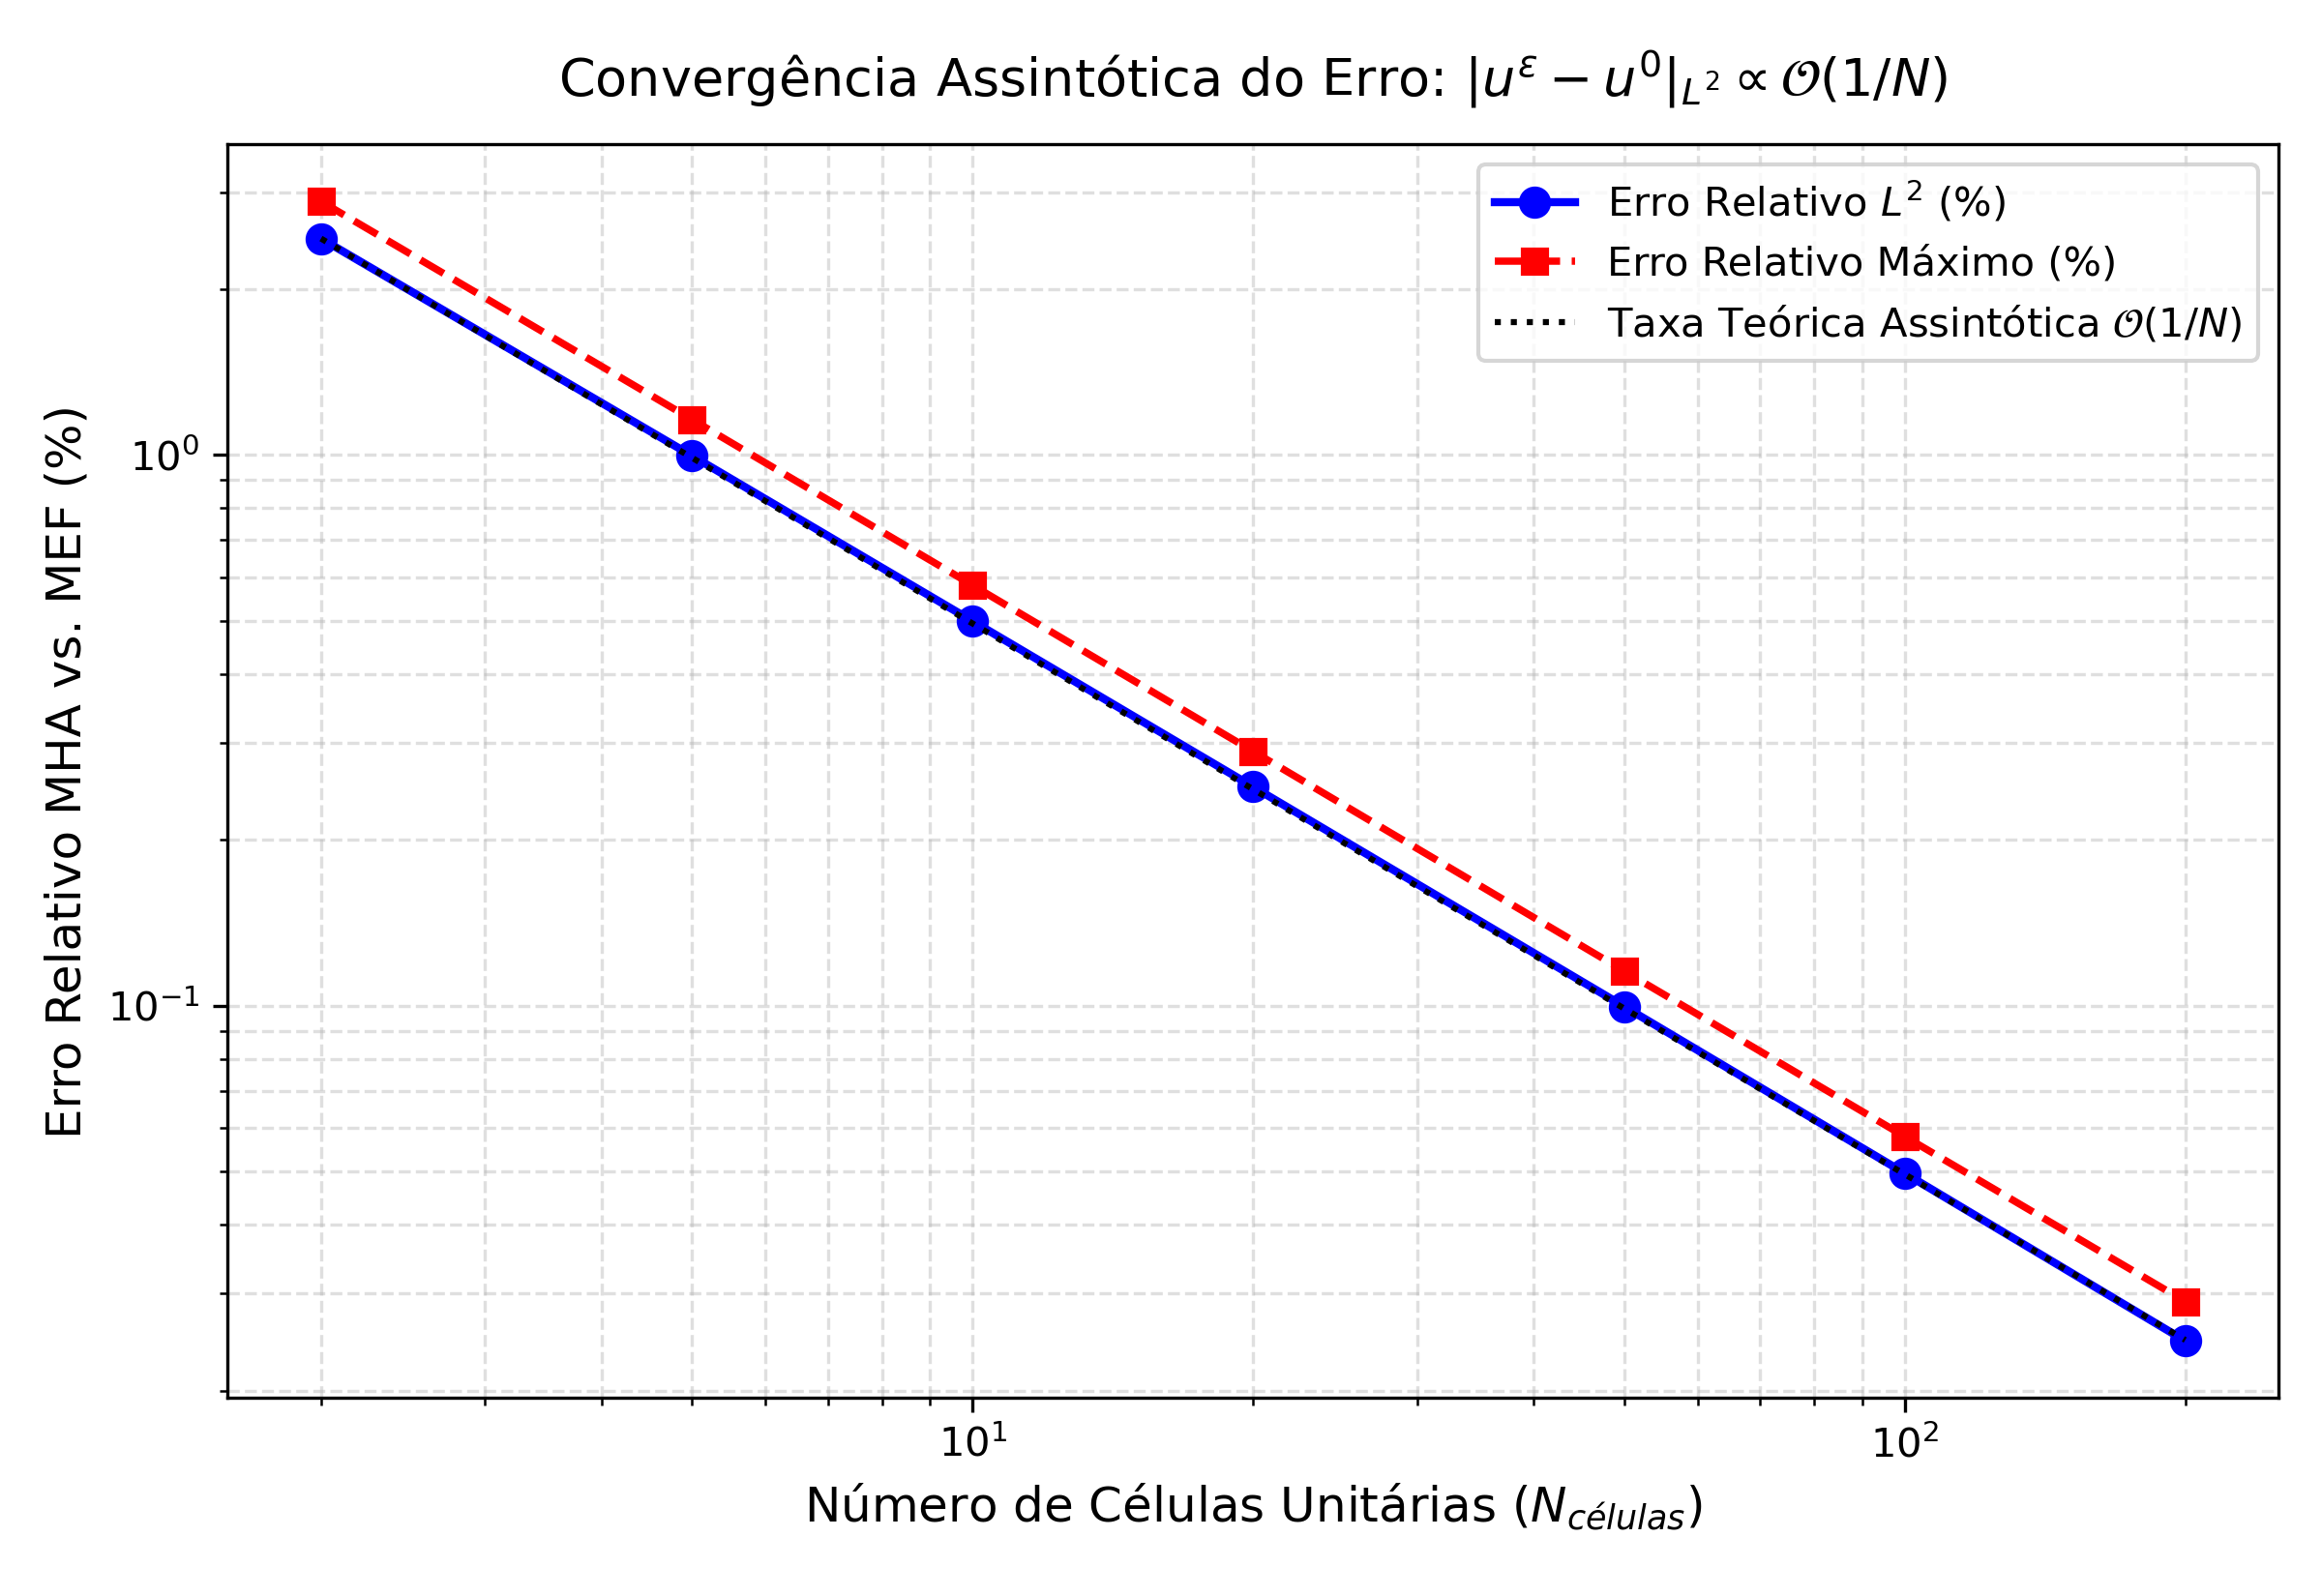
\includegraphics[width=0.85\textwidth]{../Imagens/convergencia_assintotica_erro.png}
\caption{Convergencia assintotica do erro $E_{L^2}$ em funcao do numero de celulas periodicas.}
\label{fig:convergencia_erro}
\end{figure}

\subsection{Discussão sobre Eficiência Estrutural e Custo Computacional}


A implementação computacional detalhada (classe \texttt{PeriodicProperty}, mapeamento periódico, instanciação dos campos) é descrita na Seção 4.3 do Capítulo 4. A presente seção apresenta os resultados de desempenho obtidos com essa implementação.
Para além do rigor matemático, a análise de convergência traz à tona a enorme vantagem computacional que a homogeneização assintótica confere aos projetos de engenharia.

Em termos práticos, para resolver numericamente o cilindro bimetálico com $N_{\text{cel}} = 200$ (composto por $400$ subcamadas elásticas ultrafinas de espessura de apenas $5,0 \, \mu\text{m}$), o Método dos Elementos Finitos Detalhado (MEF-D) exige uma malha radial extremamente fina para garantir o alinhamento de nós discutido no Capítulo 4. A discretização radial requerida de $4.000$ divisões gera um sistema linear com \textbf{$80.000$ triângulos discretos}, demandando um esforço computacional e de memória de CPU consideráveis para a montagem de matrizes de rigidez altamente oscilatórias.

Em contrapartida, o Método de Homogeneização Assintótica (MHA) contorna essa sobrecarga operacional de forma extremamente elegante:
1. O problema local de célula (unidimensional) é integrado analiticamente uma única vez para obter os coeficientes efetivos $[\hat{\mathcal{C}}]$, requerendo frações de segundo para ser computado;
2. O solucionador de elementos finitos macroscópico resolve o vaso como um meio contínuo homogêneo ortotrópico equivalente, eliminando a necessidade de refinar a malha para rastrear interfaces individuais. Uma malha simples e rápida com poucos graus de liberdade é suficiente para capturar a curva suave global.

Como demonstrado pela Tabela~\ref{tab:convergencia_erros}, a aproximação elástica obtida por essa abordagem simplificada MHA carrega uma divergência global de energia elástica de \textbf{apenas $0,025\%$} frente à simulação detalhada de $400$ camadas. Esse patamar é totalmente desprezível para fins práticos de engenharia, consolidando o MHA como uma ferramenta indispensável, precisa e assintoticamente exata para o projeto, análise de fadiga e otimização mecânica de vasos de pressão e cascas multicamadas de alta periodicidade.

\begin{quadro}[htbp]
\centering
\caption{Comparação de Desempenho Computacional e Precisão: MEF Heterogêneo vs. MHA Homogeneizado ($P_{int} = 30\text{ MPa}$, $V_1 = 0{,}50$).}
\label{tab:comparativo_mef_mha}
\resizebox{\textwidth}{!}{%
\begin{tabular}{cc|cc|ccc|ccc}
\hline
\textbf{$N_{cél}$} & \textbf{Camadas} & \textbf{DOFs MEF} & \textbf{DOFs MHA} & \textbf{Tempo MEF (s)} & \textbf{Tempo MHA (s)} & \textbf{Redução (\%)} & \textbf{Speedup} & \textbf{Erro Máx. (\%)} & \textbf{Erro $L^2$ (\%)} \\
\hline
2 & 4 & 198 & 682 &  0.007 &  0.010 & \textbf{-35.2\%} &   0.7x &  2.88\% &  2.47\% \\
5 & 10 & 462 & 682 &  0.008 &  0.010 & \textbf{-28.0\%} &   0.8x &  1.16\% &  1.00\% \\
10 & 20 & 902 & 682 &  0.014 &  0.010 & \textbf{ 31.1\%} &   1.5x &  0.58\% &  0.50\% \\
20 & 40 & 1,782 & 682 &  0.024 &  0.010 & \textbf{ 58.6\%} &   2.4x &  0.29\% &  0.25\% \\
50 & 100 & 4,422 & 682 &  0.058 &  0.010 & \textbf{ 82.7\%} &   5.8x &  0.12\% &  0.10\% \\
100 & 200 & 8,822 & 682 &  0.114 &  0.010 & \textbf{ 91.3\%} &  11.5x &  0.06\% &  0.05\% \\
200 & 400 & 17,622 & 682 &  0.250 &  0.010 & \textbf{ 96.0\%} &  25.1x &  0.03\% &  0.02\% \\
\hline
\end{tabular}%
}
\end{quadro}


\begin{figure}[htbp]
\centering
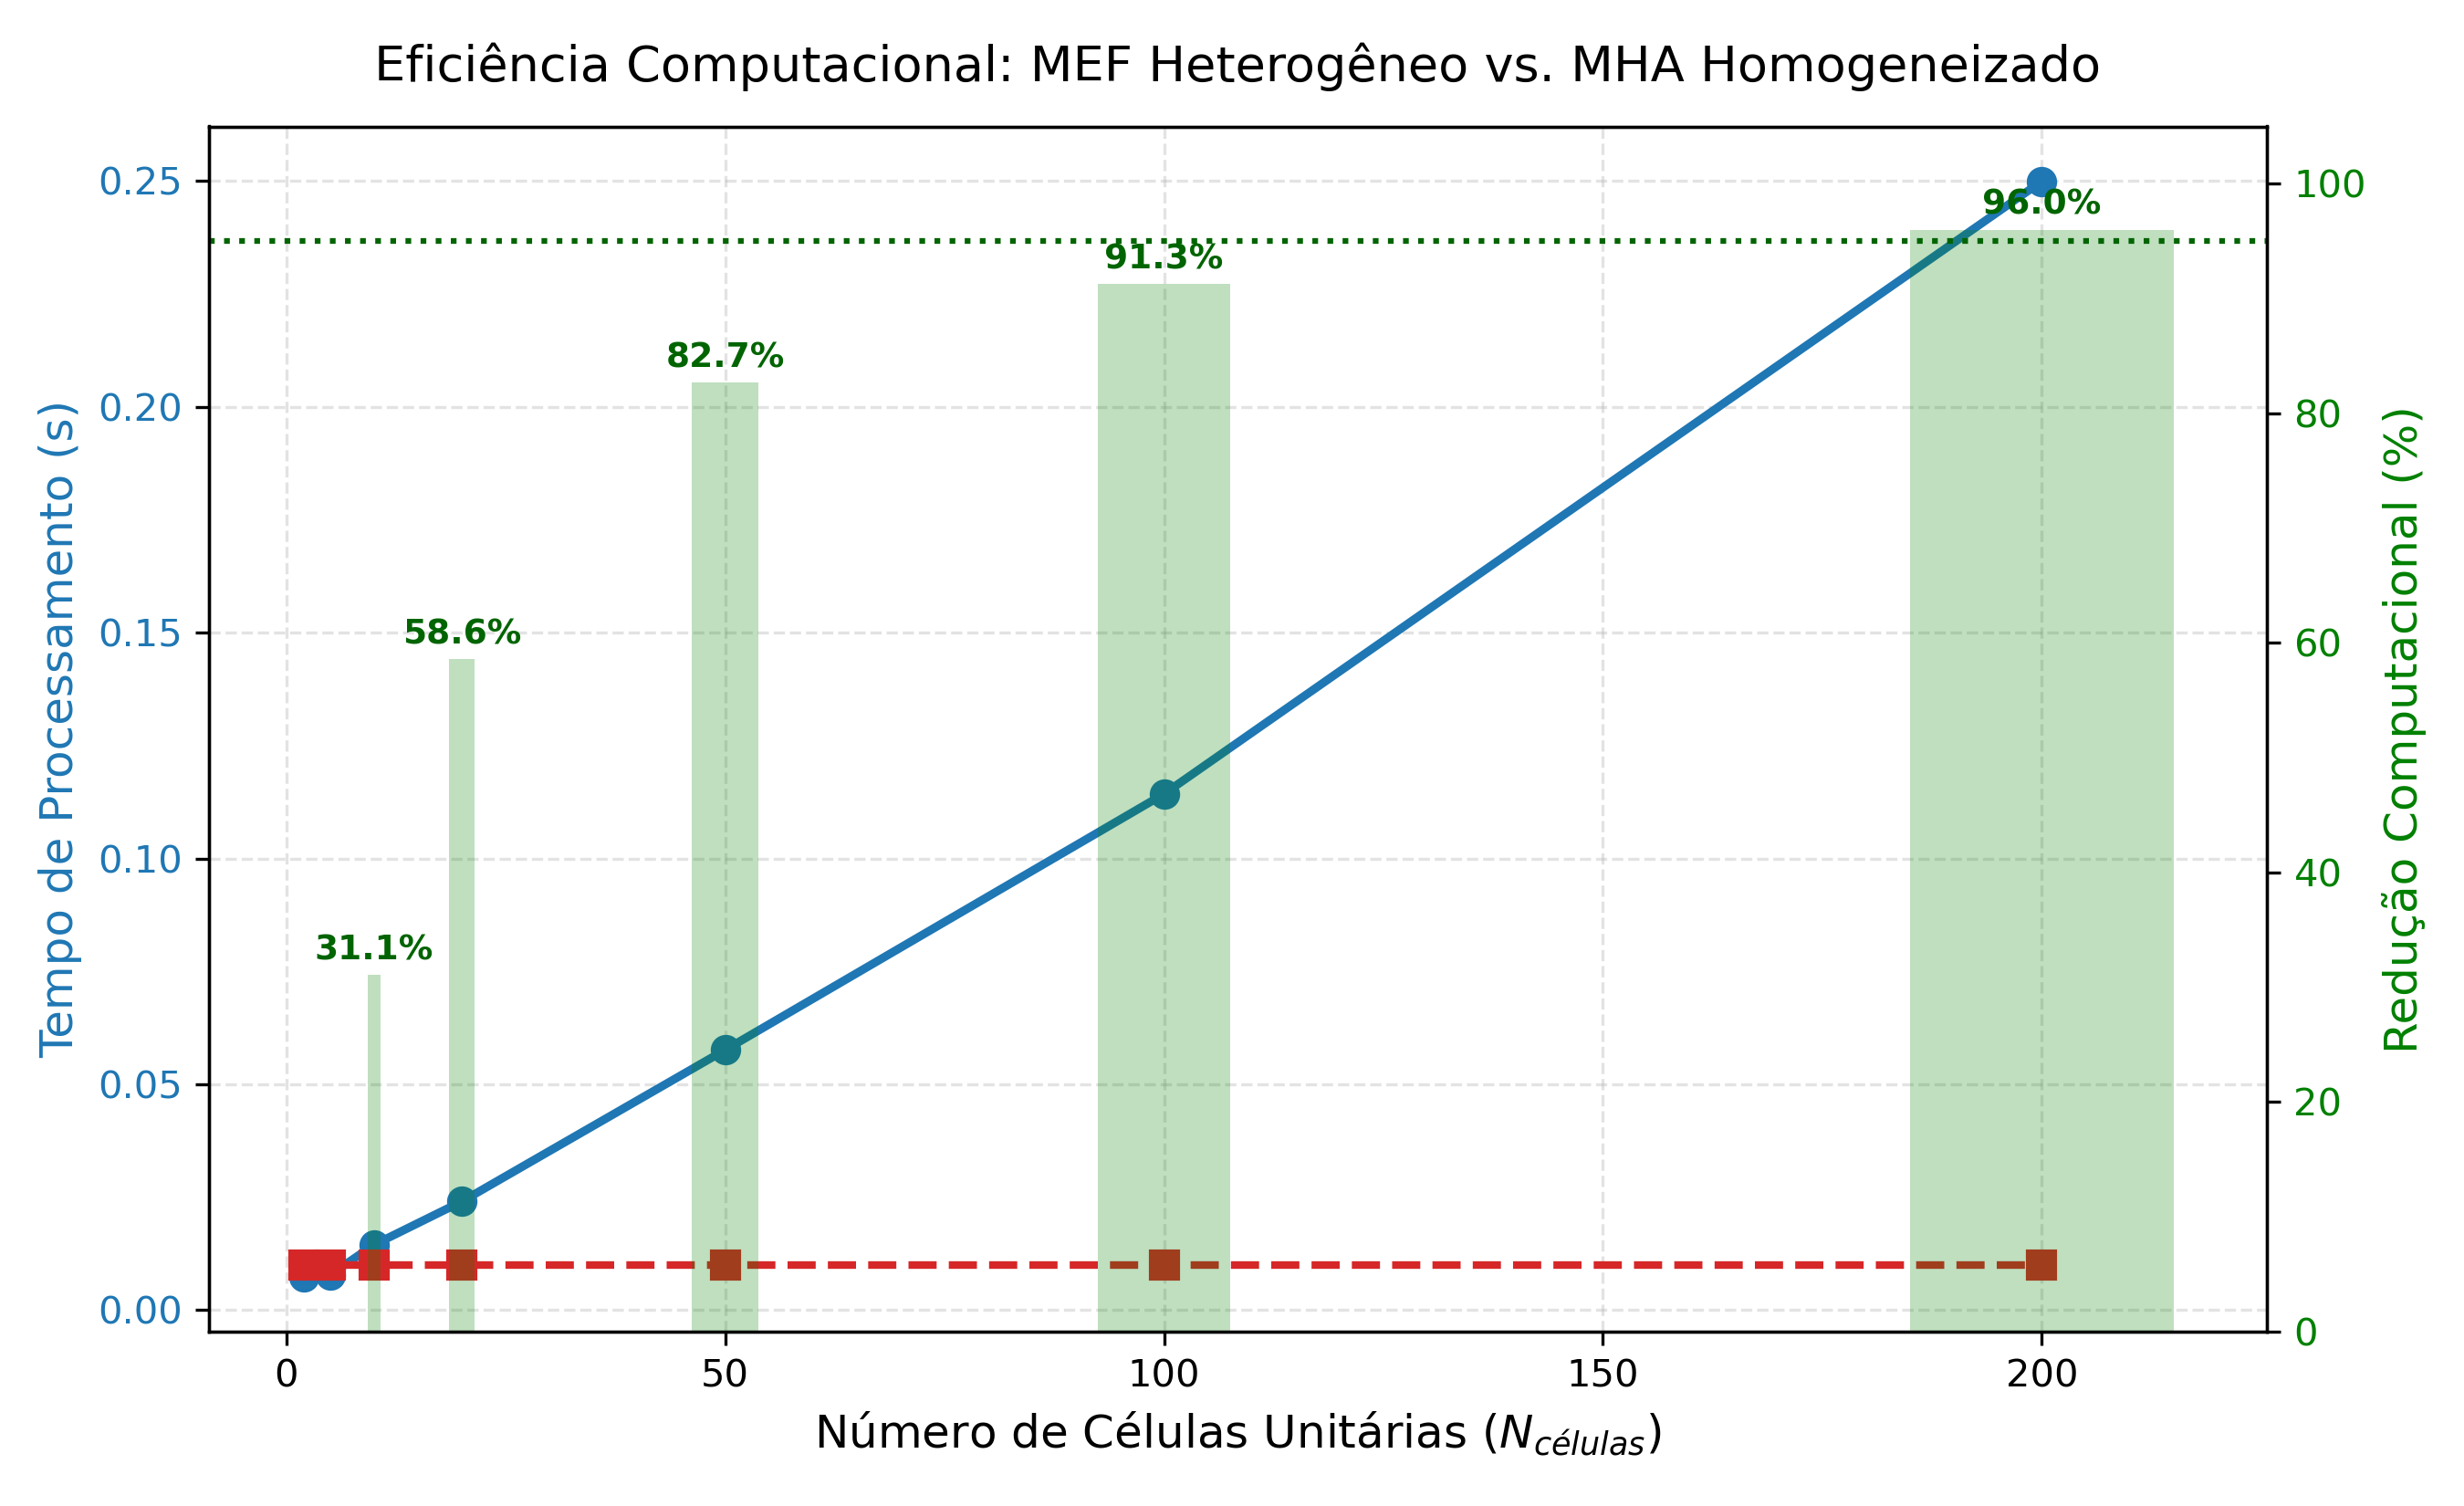
\includegraphics[width=0.85\textwidth]{../Imagens/bench_tempos_e_reducao.png}
\caption{Benchmark de tempos de execucao e reducao percentual de DOFs: MEF heterogeneo vs. MHA homogeneizado.}
\label{fig:bench_tempos}
\end{figure}



\section{Análise de Eficiência Mecânica e Resistência Específica}\label{sec:eficiencia_mecanica}

A avaliação do desempenho de um vaso de pressão de alta performance para aplicações industriais e automotivas não deve limitar-se à análise isolada da capacidade de suporte de carga ou da tensão máxima admissível. Conforme enfatizado pela literatura clássica de materiais compósitos e estruturas de peso reduzido, o critério definidor de eficiência estrutural reside na avaliação do comportamento mecânico \textbf{normalizado por unidade de massa}, expressa através da \textbf{Resistência Específica} ($W_g = \sigma_y / \hat{\rho}$) e da \textbf{Rigidez Específica} ($K_g = \hat{E} / \hat{\rho}$).

Esta seção quantifica os ganhos de eficiência mecânica e otimização estrutural proporcionados pela hibridização bimetálica periódica (Aço Carbono / Liga de Alumínio, fração volumétrica $V_1 = V_2 = 0,5$), confrontando a solução multicamadas com as configurações homogêneas fabricadas puramente em Aço Carbono e puramente em Liga de Alumínio.

\subsection{Densidade Equivalente e Alívio de Massa}

A densidade volumétrica macroscópica equivalente ($\hat{\rho}$) de um meio periódico heterogêneo é governada de forma exata e puramente aditiva pela Regra das Misturas simples:
\begin{equation}
  \hat{\rho} = V_1 \rho_{\text{aço}} + V_2 \rho_{\text{alu}} = 0,5 (7800 \, \text{kg/m}^3) + 0,5 (2700 \, \text{kg/m}^3) = 5250 \, \text{kg/m}^3
  \label{eq:densidade_efetiva_sec55}
\end{equation}

Para os raios de projeto ($R_{\text{int}} = 9,0 \, \text{mm}$ e $R_{\text{ext}} = 11,0 \, \text{mm}$), a área da seção transversal do costado do vaso equivale a $A_{\text{wall}} = \pi (R_{\text{ext}}^2 - R_{\text{int}}^2) = \pi (11,0^2 - 9,0^2) \approx 125,66 \, \text{mm}^2$. A massa linear resultante $M_{\text{linear}} = A_{\text{wall}} \hat{\rho}$, expressa em quilogramas por metro de comprimento axial (convertendo-se $A_{\text{wall}}$ para $\text{m}^2$ e mantendo-se $\hat{\rho}$ em $\text{kg/m}^3$), é sumarizada abaixo para cada uma das três configurações estruturais:
\begin{itemize}
  \item \textbf{Cilindro Homogêneo 100\% Aço Carbono:} $M_{\text{linear}} = 0,9802 \, \text{kg/m}$;
  \item \textbf{Cilindro Homogêneo 100\% Liga de Alumínio:} $M_{\text{linear}} = 0,3393 \, \text{kg/m}$;
  \item \textbf{Cilindro Multicamadas Bimetálico (MHA/MEF):} $M_{\text{linear}} = 0,6597 \, \text{kg/m}$.
\end{itemize}

Os valores absolutos são naturalmente modestos porque o domínio é analisado na escala de milímetros do modelo numérico ($R_{\text{int}} = 9,0 \, \text{mm}$); o indicador relevante para o projeto é a razão entre configurações, que é invariante a essa escala geométrica.

Conforme demonstrado analiticamente, a substituição do projeto puramente metálico em aço pela solução bimetálica hibridizada proporciona um \textbf{alívio direto de massa de $32,69\%$}. Essa redução de peso por metro linear representa um ganho substancial para o transporte, manuseio e montagem de reservatórios de grande porte de armazenamento de fluidos comprimidos.

\subsection{Avaliação da Eficiência Estrutural e Fatores de Segurança}

Para comparar o aproveitamento mecânico da matéria-prima em cada configuração sob a pressão interna de projeto de $30 \, \text{MPa}$ ($3,0 \times 10^7 \, \text{Pa}$), define-se o \textbf{Índice de Eficiência de Suporte de Carga por Unidade de Massa} ($W_{\text{ef}}$). Como a pressão de projeto é idêntica nas três configurações, a razão $P_{\text{int}}/M_{\text{linear}}$ não discrimina o desempenho do material: ela é simplesmente o inverso da massa linear. Adota-se, portanto, a pressão de início de escoamento da configuração, $P_y$, de modo que o índice meça quanta pressão o costado suporta ainda em regime elástico por unidade de massa:
\begin{equation}
  W_{\text{ef}} = \frac{P_y}{M_{\text{linear}}}, \qquad
  P_y = p \min_{k} \left( \frac{\sigma_{y,k}}{\sigma_{\text{VM},k}^{\text{máx}}} \right) = p \, \text{FS}_{\min}
  \quad [\text{MPa} \cdot \text{m/kg}]
  \label{eq:indice_eficiencia_massa}
\end{equation}

em que $\sigma_{y,k}$ é o limite de escoamento e $\sigma_{\text{VM},k}^{\text{máx}}$ a tensão equivalente de Von Mises máxima da fase $k$ sob a pressão de projeto $p$. A Tabela~\ref{tab:comparativo_eficiencia} apresenta o estudo comparativo das métricas de desempenho elástico, tensões de Von Mises máximas, fatores de segurança locais contra escoamento e massas lineares, e a Tabela~\ref{tab:indice_eficiencia_massa} consolida o índice $W_{\text{ef}}$ resultante para as três configurações de vaso de pressão sob estudo.

\begin{quadro}[htbp]
  \centering
  \caption{Estudo comparativo de eficiência estrutural, tensões equivalentes de Von Mises, fatores de segurança e alívio de massa sob pressão de projeto de $30 \, \text{MPa}$.}
  \label{tab:comparativo_eficiencia}
  \begin{tabular}{l c c c c}
    \hline
    \textbf{Configuração Estrutural} & \textbf{Densidade ($\text{kg/m}^3$)} & \textbf{Massa Linear ($\text{kg/m}$)} & \textbf{Tensão $\sigma_{\text{VM}}^{\text{máx}}$ ($\text{MPa}$)} & \textbf{Fator de Segurança ($\text{FS}$)} \\ \hline
    100\% Aço Carbono & $7800$ & $0,9802$ & $159,05$ & $2,51$ \\ \hline
    100\% Liga de Alumínio & $2700$ & $0,3393$ & $158,53$ & $1,70$ \\ \hline
    Bimetálico (Camada Aço) & $5250$ & $0,6597$ & $229,87$ & $1,74$ \\ \hline
    Bimetálico (Camada Alumínio) & $5250$ & $0,6597$ & $89,07$ & $3,03$ \\ \hline
  \end{tabular}
\end{quadro}

\begin{table}[htbp]
  \centering
  \caption{Pressão de início de escoamento ($P_y$) e índice de eficiência de suporte de carga por unidade de massa ($W_{\text{ef}}$) para as três configurações estruturais.}
  \label{tab:indice_eficiencia_massa}
  \begin{tabular}{l c c c c}
    \hline
    \textbf{Configuração Estrutural} & \textbf{$M_{\text{linear}}$ ($\text{kg/m}$)} & \textbf{$\text{FS}_{\min}$} & \textbf{$P_y$ ($\text{MPa}$)} & \textbf{$W_{\text{ef}}$ ($\text{MPa} \cdot \text{m/kg}$)} \\ \hline
    100\% Aço Carbono & $0,9802$ & $2,51$ & $75,45$ & $76,97$ \\ \hline
    100\% Liga de Alumínio & $0,3393$ & $1,70$ & $51,09$ & $150,59$ \\ \hline
    Bimetálico (MHA/MEF) & $0,6597$ & $1,74$ & $52,20$ & $79,13$ \\ \hline
  \end{tabular}
\end{table}

A análise rigorosa dos dados das Tabelas~\ref{tab:comparativo_eficiencia} e~\ref{tab:indice_eficiencia_massa} revela aspectos mecânicos de altíssimo valor técnico:

1. \textbf{Eficiência de Suporte de Carga por Unidade de Massa:} o vaso puramente de aço apresenta $W_{\text{ef}}^{\text{aço}} = 75,45 / 0,9802 \approx 76,97 \, \text{MPa}\cdot\text{m/kg}$, enquanto a solução bimetálica multicamadas atinge $W_{\text{ef}}^{\text{bimet}} = 52,20 / 0,6597 \approx 79,13 \, \text{MPa}\cdot\text{m/kg}$, o que corresponde a um acréscimo de apenas $2,80\%$. O cilindro de alumínio puro, por sua vez, alcança $W_{\text{ef}}^{\text{alu}} = 150,59 \, \text{MPa}\cdot\text{m/kg}$, valor $90,3\%$ superior ao do composto. Esse ordenamento é consequência direta da razão resistência/densidade dos materiais empregados ($\sigma_y/\rho = 0,100 \, \text{MPa}\cdot\text{m}^3/\text{kg}$ para o alumínio contra $0,0513 \, \text{MPa}\cdot\text{m}^3/\text{kg}$ para o aço): quando o critério de mérito é exclusivamente a resistência específica, o alumínio monolítico é imbatível e a hibridização não o supera. Além disso, o $P_y$ do composto é governado pela camada de aço ($\text{FS} = 1,74$), de modo que o índice penaliza o bimetálico precisamente pelo mecanismo que ele foi projetado para explorar — a transferência de carga para a fase mais resistente. A vantagem da solução híbrida deve, portanto, ser avaliada em conjunto com a rigidez específica e com a elevação do fator de segurança da fase de alumínio, discutidas a seguir.
2. \textbf{Distribuição Inteligente de Esforços:} Em um cilindro de alumínio puro sob $30 \, \text{MPa}$, a tensão de Von Mises de $158,53 \, \text{MPa}$ consome grande parte da capacidade do material, resultando em um fator de segurança modesto de $\text{FS} = 1,70$ frente ao seu limite de escoamento de $270 \, \text{MPa}$. Na estrutura bimetálica, as camadas de aço carbono (mais rígidas) puxam as tensões circunferenciais de tração para si ($\sigma_{\theta\theta}^{\text{aço}} = 231,33 \, \text{MPa}$), aliviando drasticamente a sobrecarga sobre o alumínio ($\sigma_{\theta\theta}^{\text{alumínio}} = 72,51 \, \text{MPa}$).
3. \textbf{Elevação do Fator de Segurança do Alumínio:} Como consequência do efeito de "cinturamento" promovido pelas subcamadas de aço, o fator de segurança da fase de alumínio no composto eleva-se para \textbf{$\text{FS} = 3,03$} (um ganho de $78,2\%$ em relação ao alumínio puro), enquanto a camada de aço, que passa a concentrar a solicitação, opera com $\text{FS} = 1,74$ e passa a governar o limite elástico da configuração.

\subsection{Rigidez Específica e Desempenho Global}

Em termos de rigidez elástica tangencial (resistência ao estufamento por expansão radial), a constante homogeneizada de Backus para o composto bimetálico equivale a $\hat{C}_{22} = 1,8093 \times 10^{11} \, \text{Pa}$ ($180,93 \, \text{GPa}$).

A razão de rigidez específica do compósito é calculada por:
\begin{equation}
  K_g^{\text{bimet}} = \frac{\hat{C}_{22}}{\hat{\rho}} = \frac{1,8093 \times 10^{11} \, \text{Pa}}{5250 \, \text{kg/m}^3} \approx 3,446 \times 10^7 \, \text{m}^2/\text{s}^2
  \label{eq:rigidez_especifica_bimet}
\end{equation}

Para o aço carbono maciço ($\mathcal{C}_{11} = 269,23 \, \text{GPa}$ e $\rho = 7800 \, \text{kg/m}^3$), a rigidez específica resulta em $K_g^{\text{aço}} \approx 3,452 \times 10^7 \, \text{m}^2/\text{s}^2$. Isso comprova que a estrutura bimetálica \textbf{preserva $99,84\%$ da rigidez específica do aço maciço}, porém fornecendo um alívio de peso de quase um terço do total da estrutura. Para a liga de alumínio ($E = 70 \, \text{GPa}$ e $\rho = 2700 \, \text{kg/m}^3$), obtém-se $K_g^{\text{alu}} \approx 2,593 \times 10^7 \, \text{m}^2/\text{s}^2$, de modo que o composto é cerca de $32,9\%$ mais rígido por unidade de massa que o alumínio monolítico. É nesse compromisso entre rigidez específica e resistência específica, e não no mérito isolado de cada um deles, que reside o ganho efetivo da hibridização periódica.

Estes resultados confirmam a plena viabilidade técnica do Método de Homogeneização Assintótica (MHA) no projeto e otimização de vasos de pressão multicamadas, demonstrando que a hibridização bimetálica periódica é uma alternativa de engenharia madura, segura e de elevada eficiência mecânica para reservatórios de alta pressão.
